\begin{figure}[!t]
\centering
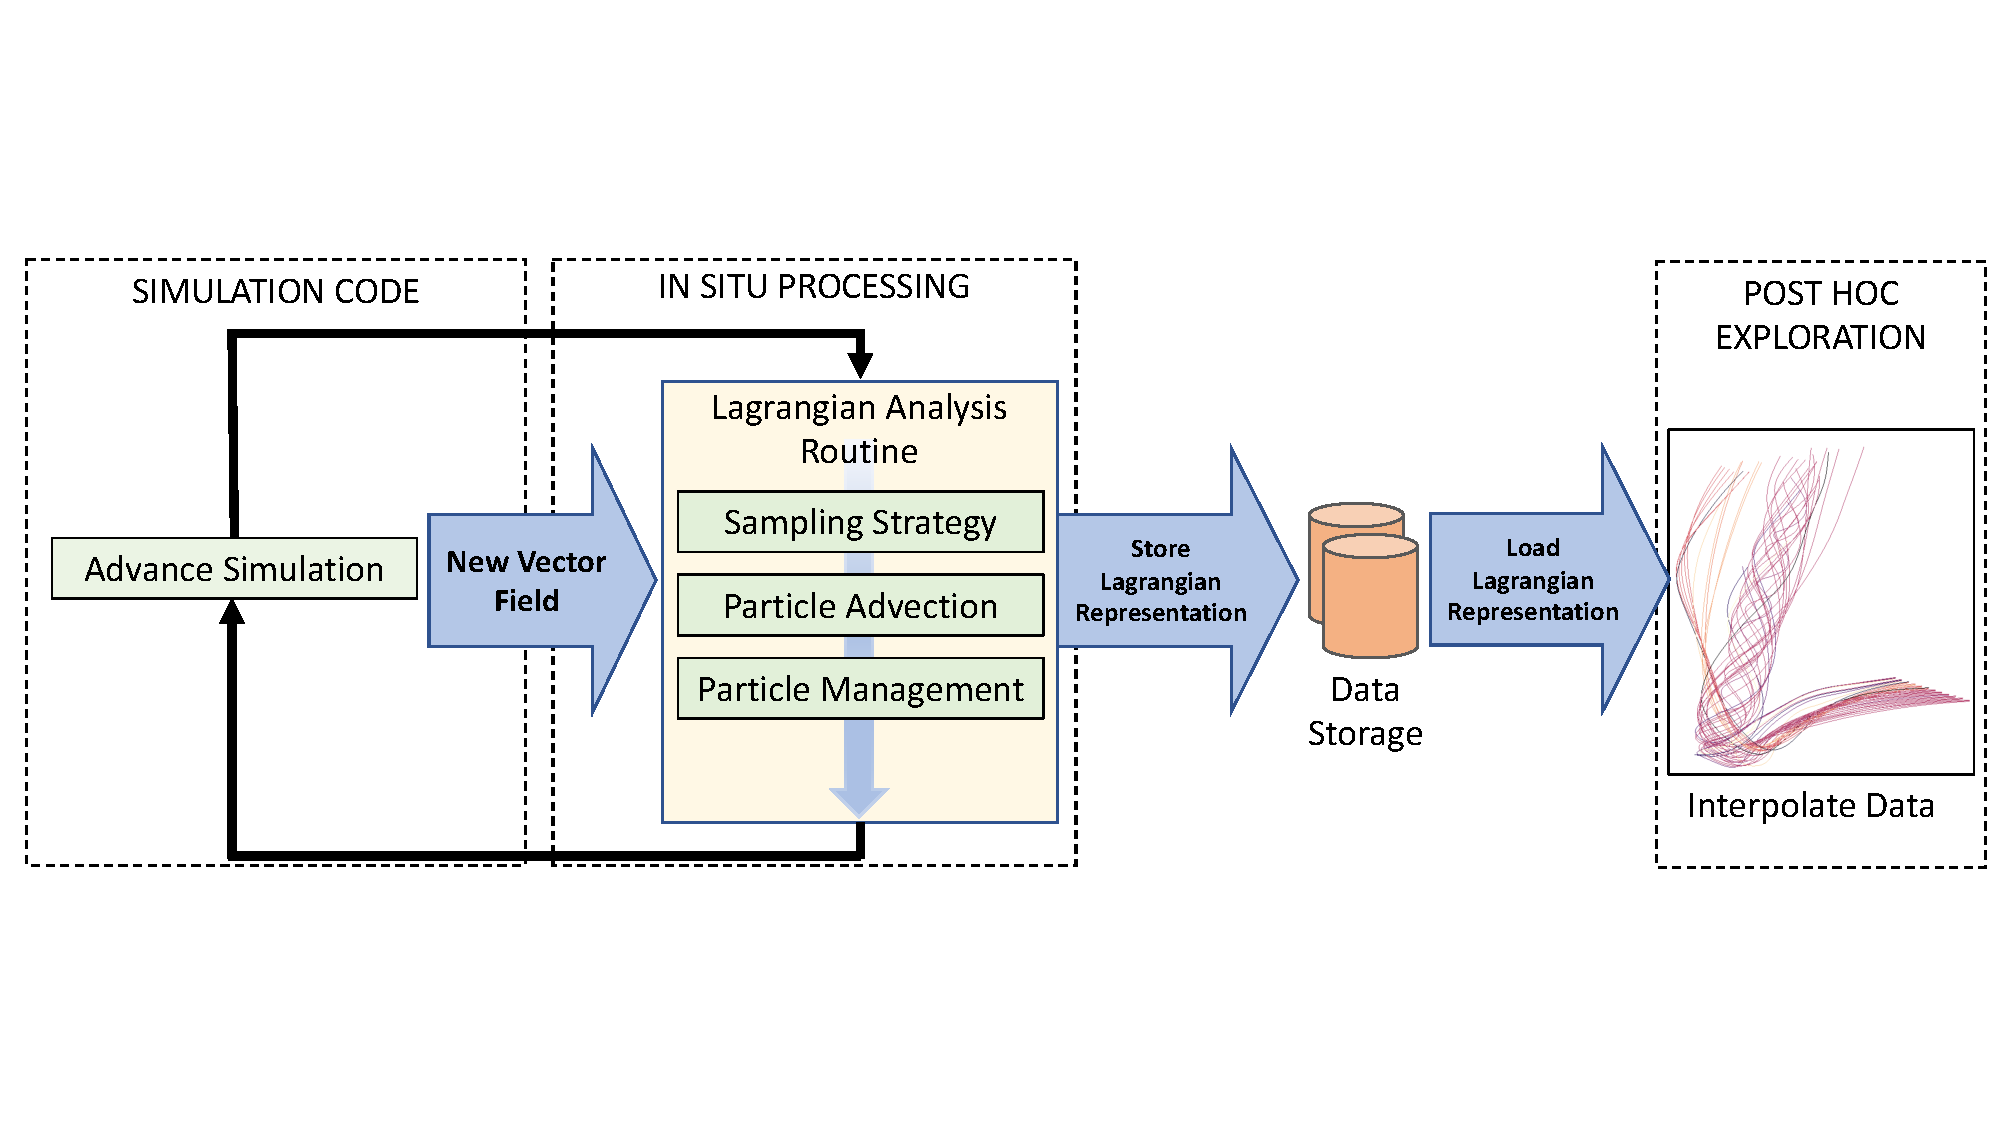
\includegraphics[width=0.9\linewidth,trim={0cm 4.3cm 0cm 4.3cm}, clip ]{Images/Schematic.pdf}
%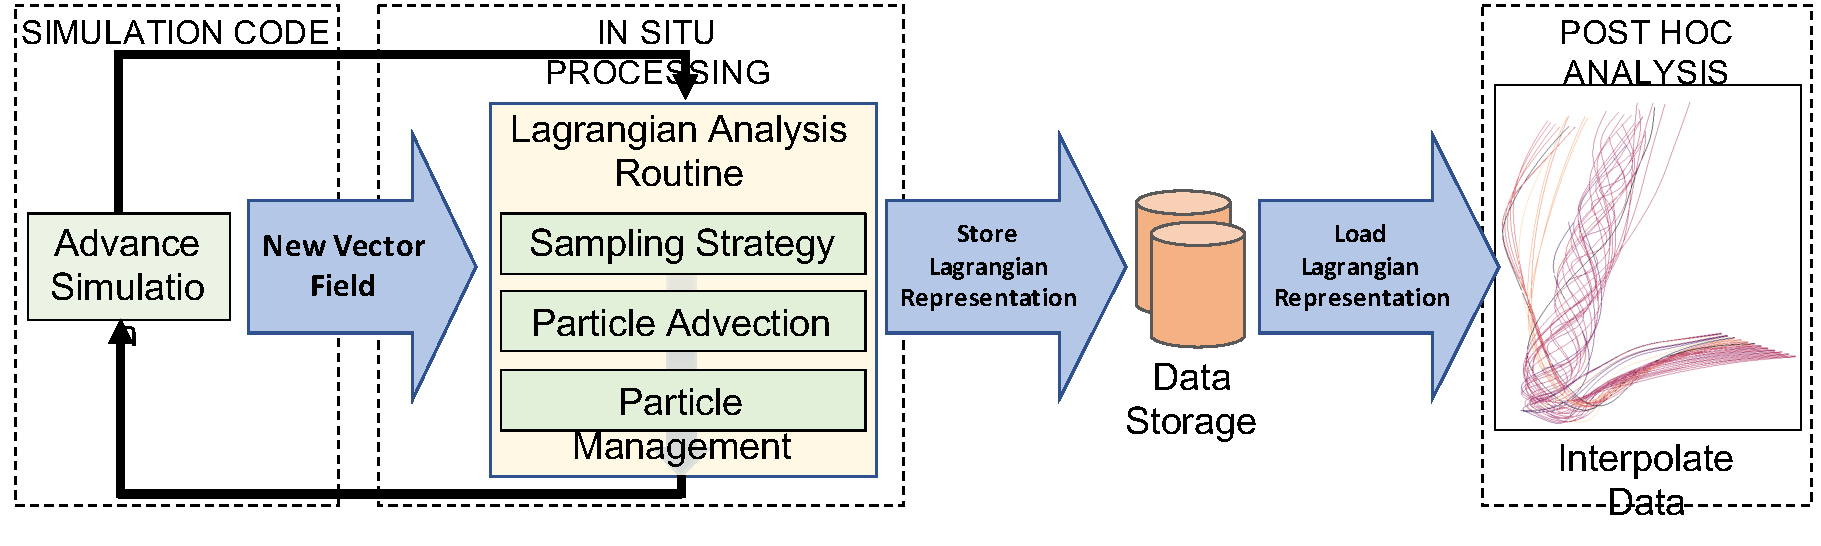
\includegraphics[width=0.9\linewidth]{Images/Schematic_Short.pdf}
\vspace{-2mm}
\caption{Schematic of the Lagrangian in situ reduction and post hoc exploration workflow.} %the simulation code with in situ processing integrated, data storage, and post hoc analysis.}
\vspace{-5mm}
\label{fig:schematic}
\end{figure}

This section describes the instantiation we consider for our study.
%
Figure~\ref{fig:schematic} shows a high-level description of the Lagrangian in situ reduction post hoc exploration (L-ISR-PHE) workflow. 
%
%There are many possible strategies for accomplishing the components within this workflow.
%
For our study, we focused on the current best practices in this space.
%
To describe our instantiation, the remainder of this section is divided based on the two phases: in situ reduction and post hoc exploration. 
%

\noindent\textbf{In Situ Reduction}
%
Both simulations we considered partitioned space amongst ranks,
with each rank owning one portion of the vector field.
Our in situ routines followed this pattern, with an
instance of our Lagrangian analysis
routine executing for each rank, accessing its portion
of the vector field.
%
Further, for both simulations we were interested in capturing time-varying vector field behavior across the entire domain.
%
Thus, for our in situ data reduction strategy, we prioritized domain coverage.
%
Similar to Agranovsky et al.~\cite{agranovsky2014improved}, we used uniform spatial sampling and a predetermined interval to store/reset particles.
%
Thus, we computed sets of temporally non-overlapping basis trajectories over the duration of the simulation.
%
Each set of basis trajectories encodes the behavior of the time-varying vector field over a specific interval of time.
%
Our particle termination followed the local Lagrangian flow map model from Sane et al.~\cite{sane2020scalable}, where particles are terminated once they reach the end of the interval or exit the block.
%
Our implementation had two main knobs that control the total data storage and quality of reconstruction: number of basis trajectories, i.e., spatial sampling resolution, and frequency of storing information to disk, i.e., storage interval.
%
The effect of these settings varies depending on the underlying vector field. 
%

We used the Ascent~\cite{Larsen2017Alpine} in situ infrastructure and VTK-m~\cite{moreland2016vtk} library to implement L-ISR. 
%
The Ascent API can be used to perform tightly-coupled integration with an application code and access various in situ analytics capabilities.
%%
The VTK-m Lagrangian filter on each rank operated independently and maintained its own list of particles.
%
We used the existing particle advection infrastructure available in VTK-m~\cite{pugmire2018performance}.
%
RK4 particle advection is implemented using VTK-m worklets (kernels) that offer performance portability by utilizing the underlying hardware accelerators.
%
In our implementation, each Lagrangian filter stored the displacement of each particle (three double), as well as its validity (one Boolean), i.e., whether the particle remained within the domain during the interval of calculation.
%
Overall, computing a Lagrangian representation increased the runtime memory cost on the simulation by approximately by four one-dimensional simulation ``fields''.
%
Simulations often have tens to hundreds of fields defined on the simulation grid, and thus, this cost would likely be acceptable for most simulations.
%
%In more complicated frameworks, it is possible to associate additional information (for example, ID, age, start location, previous locations, etc.) with each particle at the cost of higher runtime memory usage and data storage.
%

To compute a Lagrangian representation, the simulation invoked Ascent after every cycle it advanced.
%
Ascent accessed the simulation vector field data and consequently invoked the Lagrangian filter. 
%
The Lagrangian filter used the vector field to advance particles, and triggered the storage of trajectories at the end of an interval.
%
%In our implementation, following previous work~\cite{agranovsky2014improved}\cite{sane2018revisiting}\cite{sane2020scalable}, a trajectory in the Lagrangian representation is stored using a start and end location.
%
For integration, all the steps involved --- creating an instance of Ascent, specifying parameters, and invoking the VTK-m Lagrangian filter --- required only 23 lines of code (C++). % and less is a JSON input file was used.
%
%The code sample in Listing~\ref{lst:code} shows these steps. 
%

\noindent\textbf{Post Hoc Exploration}
For post hoc analysis, new particle trajectories are computed to explore the time-varying vector field. %by interpolating basis trajectories that were extracted in situ.
%
To construct new particle trajectories, we first identified which basis trajectories to follow and then performed interpolation.
%
Based on the study of accuracy of various Lagrangian-based advection schemes in~\cite{agranovsky2015subsampling}, our study employed a Delaunay triangulation to identify the neighborhood of valid basis trajectories and second-order barycentric coordinates for interpolation.
%
We used the CGAL~\cite{fabri2011cgal} library to construct and search the Delaunay triangulation.
%
After constructing new pathlines or deriving new scalar fields from the basis trajectories, we used VisIt~\cite{childs2012visit} to generate visualizations.
